\section{Materials}
\label{sec:materials}

This section describes the EPIC-KITCHENS-100 dataset, the empirical exploration that informed our preprocessing decisions, and the pre-trained checkpoints, hardware and software stack that supported the three approaches.

\subsection{Dataset and empirical exploration}
\label{sec:materials:data}

\begin{figure}[t]
    \centering
    
\includegraphics[width=0.65\textwidth]{images/collage.png}
    \caption{Qualitative overview of EPIC-KITCHENS-100 with multiple example frames illustrating different kitchens, viewpoints and activities.}
    \label{fig:dataset_collage}
\end{figure}

We use the EPIC-KITCHENS-100 dataset, focusing on the Multi-Instance Retrieval (MIR) challenge. The corpus comprises trimmed egocentric action segments paired with English narrations, recorded with head-mounted cameras in 45 kitchens and totaling 100 hours of Full-HD video. This encompasses around 20\,M frames distributed in 700 variable-length sequences with 97 verb classes and 300 noun classes~\cite{damen2022rescaling}. The retrieval split releases $67{,}217$ training segments and $9{,}668$ test segments paired with $3{,}842$ unique narrations on the test side. Ground-truth relevance is provided as the soft-label matrix released by Wray et al.~\cite{wray2021semantic} alongside the dataset. The \emph{test} relevance matrix is held out by the organizers and available exclusively through the Codabench grader, restricting offline metric computation to the public training and validation splits. Figure~\ref{fig:dataset_collage} illustrates the visual diversity of the corpus.

\paragraph{Video- and image-level statistics.}
The official \texttt{EPIC\_100\_video\_info.csv} reports a mean video duration of $\approx 514$\,s (std.\ 599\,s) across the 700 recordings, ranging from $\sim$10\,s clips to long sessions exceeding one hour, and an average frame rate of $55.9$\,fps with most recordings at 50 or 59.94\,fps. Videos are predominantly Full HD ($1920\times 1080$): $694$ of $700$ recordings use this resolution, yielding an average of $\approx 2.07\times 10^{6}$ pixels per RGB frame; appearance statistics computed on a uniform sample of $1{,}000$ training frames yield mean RGB intensities of $\approx (0.44, 0.37, 0.36)$ and per-channel standard deviation $\approx 0.21$ on a $0$--$1$ scale, summarizing typical kitchen illumination levels.

\begin{figure}[t]
    \centering
    \begin{subfigure}[b]{0.31\textwidth}
        \centering
        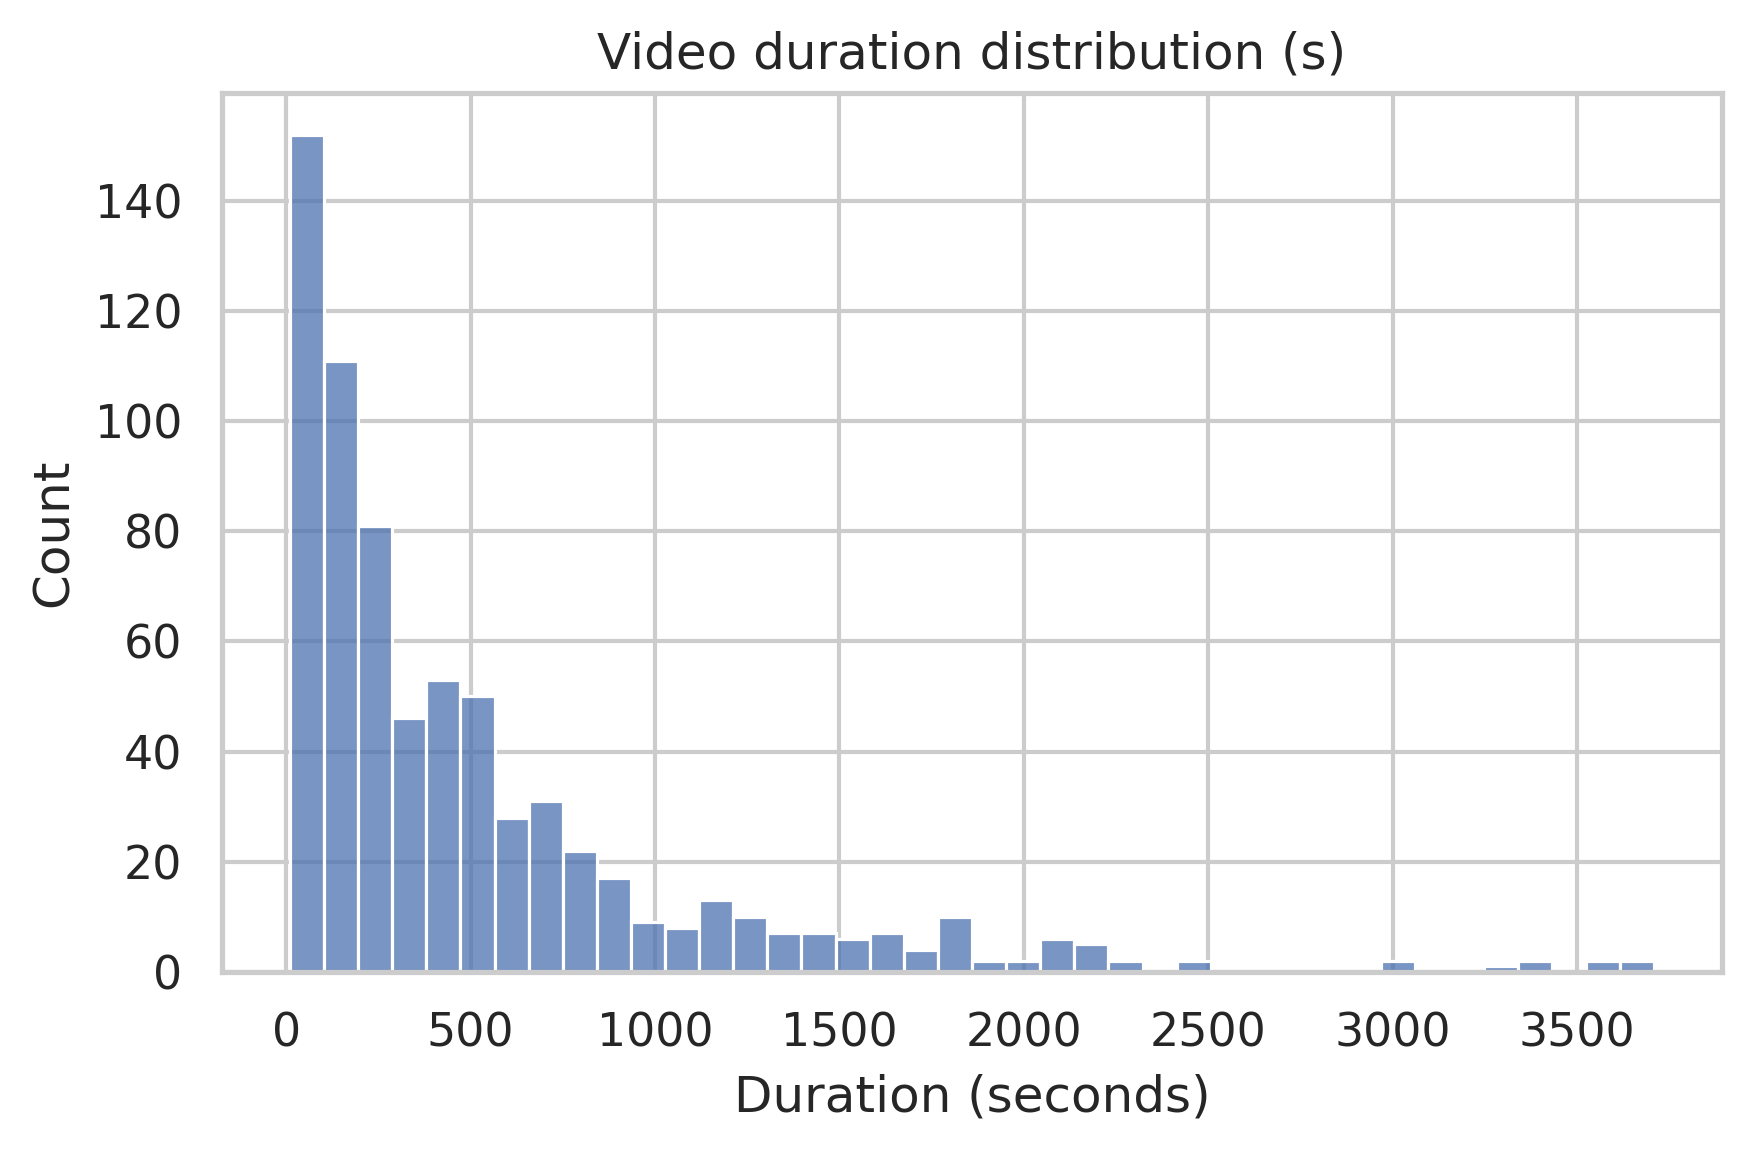
\includegraphics[width=\textwidth]{images/video_duration_hist.png}
        \caption{Video duration.}
        \label{fig:video_duration_hist}
    \end{subfigure}
    \hspace{0.01\textwidth}
    \begin{subfigure}[b]{0.31\textwidth}
        \centering
        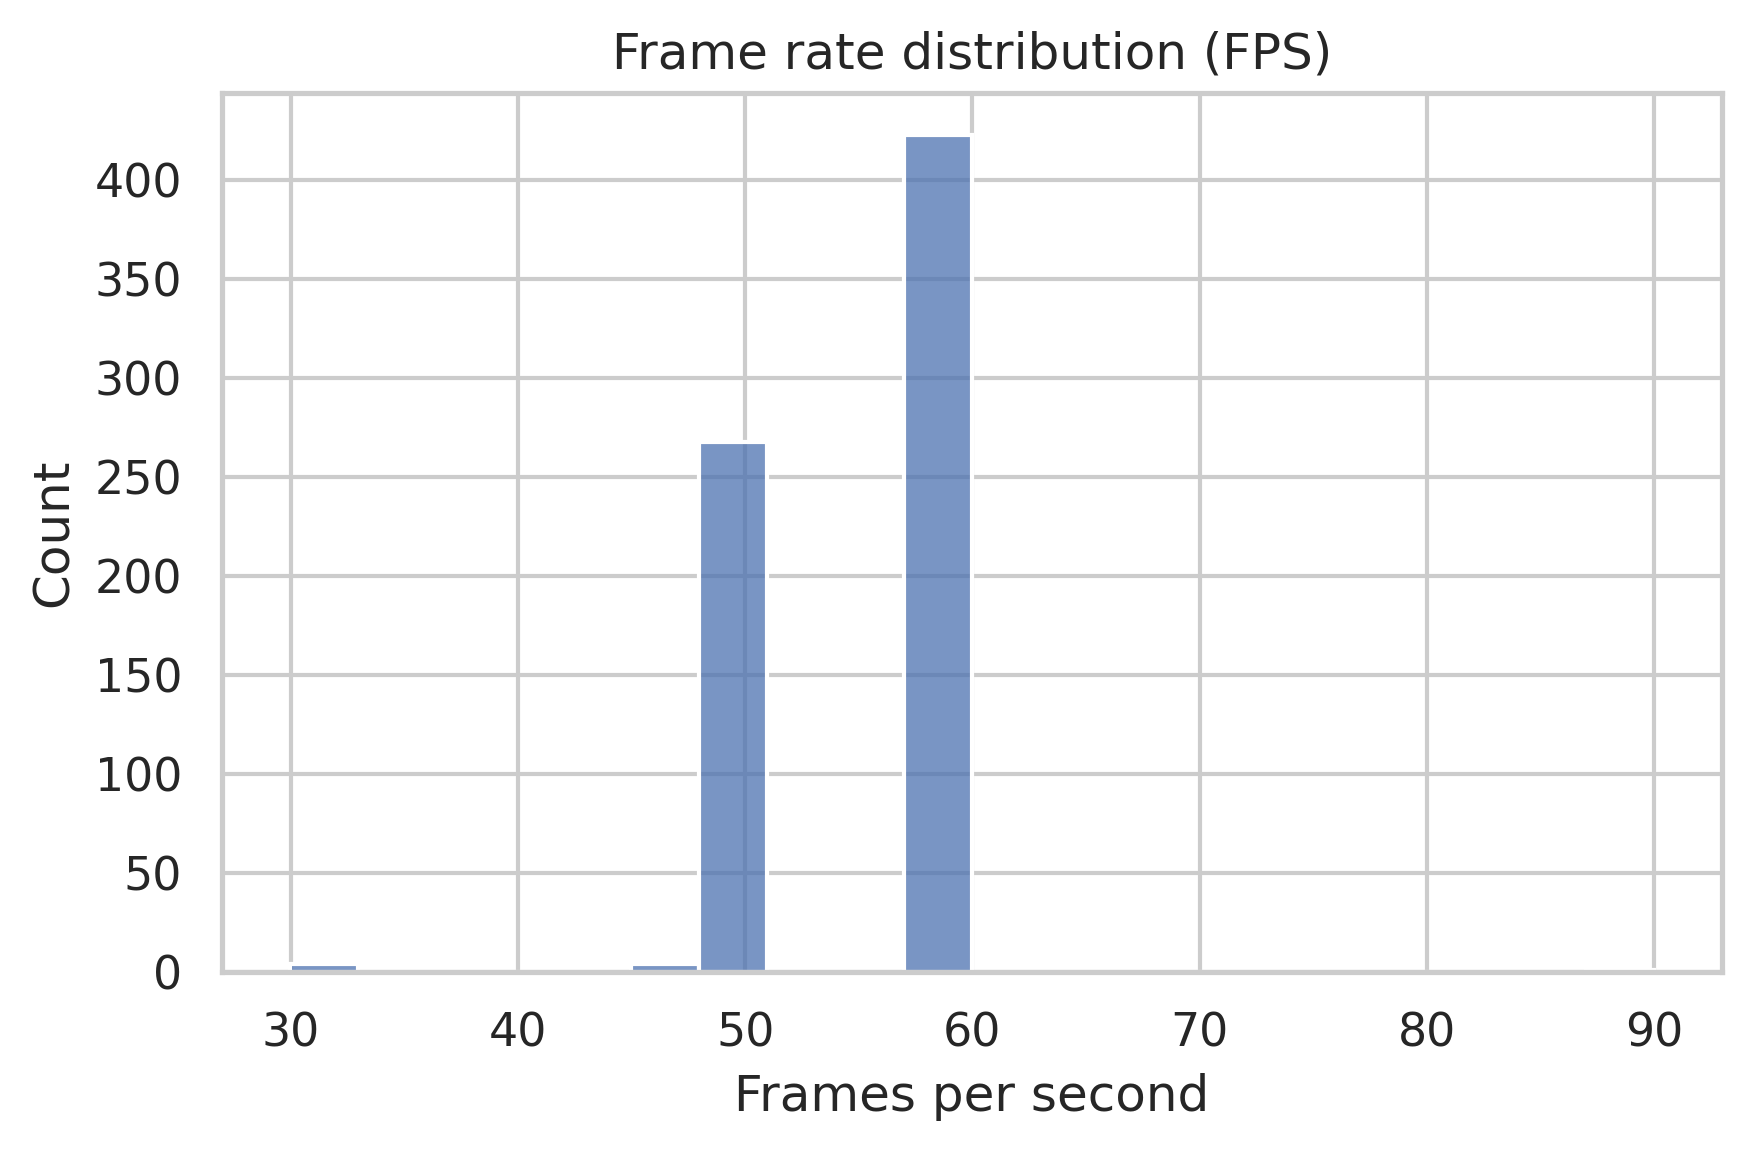
\includegraphics[width=\textwidth]{images/fps_hist.png}
        \caption{Frame rate.}
        \label{fig:fps_hist}
    \end{subfigure}
    \hspace{0.01\textwidth}
    \begin{subfigure}[b]{0.32\textwidth}
        \centering
        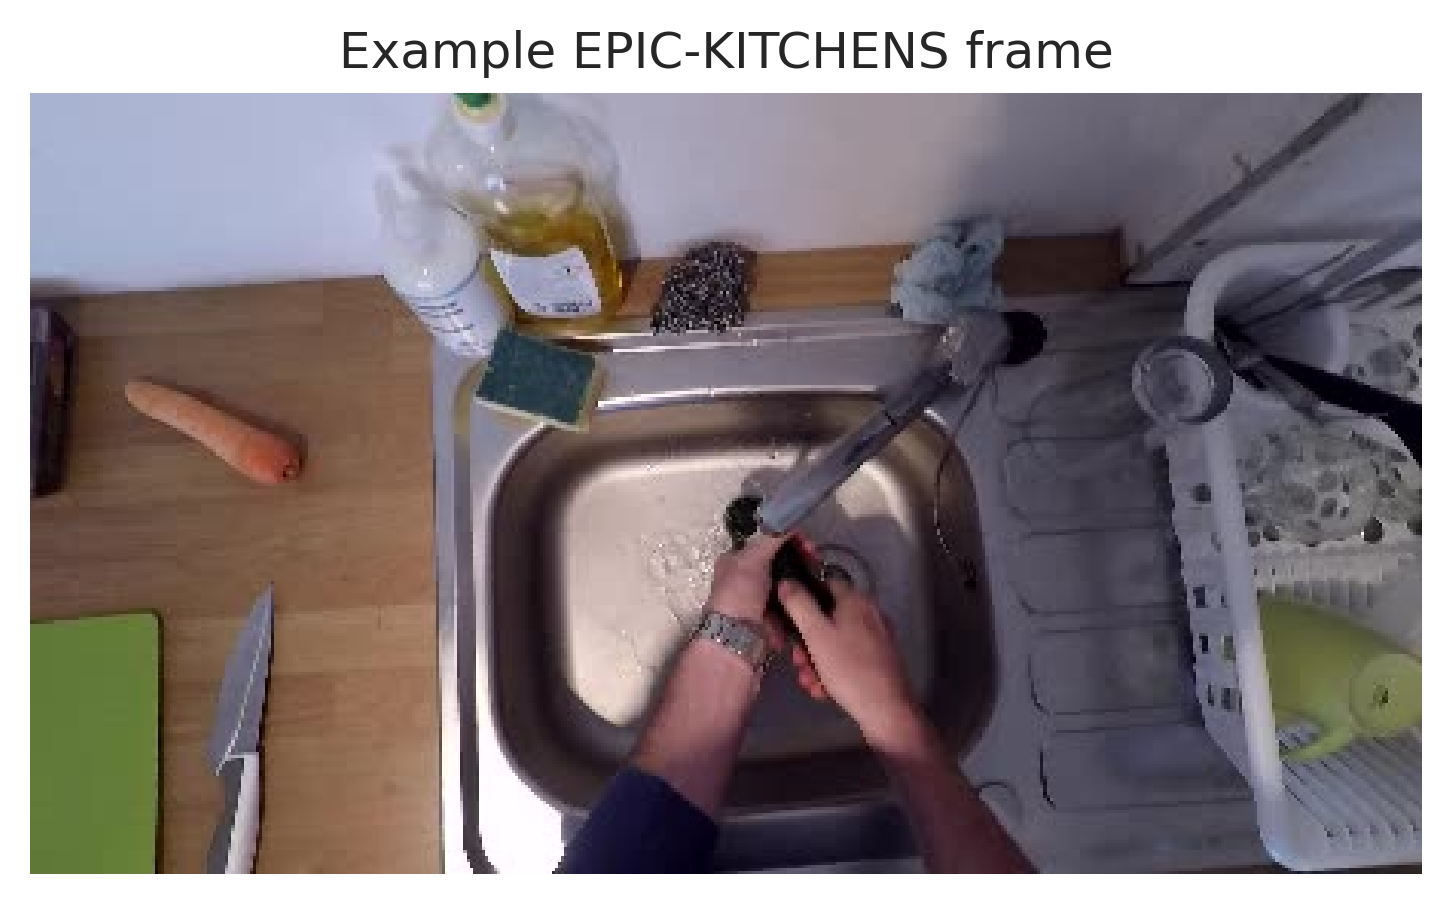
\includegraphics[width=\textwidth]{images/example_frame.png}
        \caption{Example frame.}
        \label{fig:example_frame}
    \end{subfigure}
    \caption{Video-level distributions of duration (s) and frame rate (fps) and a representative training frame illustrating the egocentric viewpoint and typical kitchen clutter.}
    \label{fig:video_stats}
\end{figure}

\paragraph{Segment-level statistics for MIR.}
Segment durations are computed from the retrieval annotation files as $\texttt{dur} = (\texttt{stop\_frame} - \texttt{start\_frame} + 1)/\texttt{fps}$. For the $67{,}217$ training segments, the mean is $3.18$\,s (std.\ $5.53$, median $1.6$, IQR $[1.0, 3.18]$\,s), confirming that most clips are very short while a long tail of extended actions reaches $\sim 297$\,s. This long tail motivates the choice of clip length used by our AVION-based fine-tuning pipeline (Section~\ref{sec:methods:avion}), where short default clips of 8 frames are augmented at test time to 32 frames for richer temporal context.

\subsection{Pre-trained checkpoints, hardware and software}
\label{sec:materials:stack}

Each approach reuses publicly released checkpoints. Approaches~1 and~2 operate on pre-extracted features and were executed on a single NVIDIA T4 (16\,GB) provided by Google Colab, using the JPoSE and MMEN encoders distributed by Wray et al.~\cite{wray2019jpose} together with the MI-MM checkpoint and S3D-HowTo100M features released alongside MIL-NCE~\cite{miech2020milnce}. Approach~3 fine-tunes a ViT-L/14 backbone from the AVION pre-train checkpoint of Zhao and Kr\"ahenb\"uhl~\cite{zhao2023avion}. It was deployed on a single NVIDIA A100 (40\,GB), with gradient checkpointing, the \texttt{use-fast-conv1} optimization of AVION and FlashAttention~\cite{dao2022flashattention} when available, halving attention memory at no accuracy cost, AdamW optimization ~\cite{loshchilov2019adamw}, a base learning rate of $2\times 10^{-5}$ and batch size $48$. Approach~3 also requires staging $\approx 720$\,GB of EK-100 video chunks (320p, 15\,s, 30\,fps, libx264) on persistent storage, together with the EK-100 retrieval annotations and the public training relevancy matrix~\cite{wray2021semantic}. As mentioned, the test relevancy matrix is held out by the organizers and not used at any stage. The implementation is built on PyTorch 2.4.1 (CUDA 12.1) with the standard vision--language components (\texttt{open\_clip\_torch}, \texttt{openai/CLIP}, \texttt{transformers}, \texttt{timm}), \texttt{decord} for video I/O, and \texttt{numpy}/\texttt{scipy.sparse} for the ensemble and re-ranking of Approach~2. Submissions are packaged as pickle protocol 2 with a numpy namespace compatibility shim required by the Codabench grader. The SMS-Loss code used in Approach~3 is a patched fork of the public release~\cite{wang2024smsloss_repo,wang2024symmetricmultisimilaritylossepickitchens100} that fixes a small number of bugs preventing stable end-to-end runs on EK-100 (tuple unpacking in the gradient-accumulation branch, an undefined \texttt{accum\_freq} reference replaced by \texttt{update\_freq}, dataloader retry logic for missing or corrupt video chunks, and \texttt{module.}-prefix stripping when loading \texttt{DataParallel}-wrapped checkpoints).
